\subsection{Différents algorithmes de synthèse d'ouverture}
Cette section porte sur la présentation puis la comparaison des différents algorithmes de formation d'image de radar à synthèse d'ouverture. L'objectif est de réaliser un choix sur l'algorithme que nous allons utiliser. ...........
\subsubsection{Range-Doppler Algorithm (RDA)}
L'algorithme Range-Doppler (RDA) est une méthode très répandue en formation d'image SAR, développée à la fin des années 1970. Son principe repose sur deux étapes principales : la compression en distance pour obtenir une résolution fine en portée, suivie d'une transformée de Fourier Doppler en azimut permettant de séparer puis de compresser les différentes fréquences Doppler induites par le mouvement relatif radar-cible. Le RDA corrige ensuite la migration des cellules de portée via une interpolation (RCMC) dans le domaine fréquentiel. Cette approche exploite la séparable approximation entre le traitement en distance et en azimut, offrant un bon compromis entre efficacité de calcul et qualité d'image, mais nécessite une trajectoire quasi-linéaire et stable pour conserver la cohérence de phase nécessaire à la formation précise des images. \cite{krieger1998digital}
\paragraph{La compresion en distance}
L'opération de compression en distance dans les algorithmes de traitement SAR est uen étape qui consiste à améliorer la résolution en distance de notre système par une technique de traitement. \\
Pour expliquer ce principe, on considère un radar pulsée non modulé en fréquence. 
\noindent On part de l'expression classique 
\[ 
\tau = \frac{2R}{c}
\]
\noindent Avec la différenciation, on obtient 
\[
\Delta R = \frac{c \Delta \tau}{2} 
\]
\noindent On a fait apparaitre ici la résolution en distance $\Delta R$ et le temps minimum pour distinguer deux impulsions $\Delta \tau$ que l'on peut transformer en $T_p$ la durée d'une impulsion, ce qui nous donne 
\begin{equation}
\label{eq: delta_r}
    \Delta R = \frac{c T_p}{2}
\end{equation}


\noindent Alors, nous faisont fasse à un dilemne: pour améliorer notre résolution spatiale, nous devons réduire la durée de notre impulsion. Seulement réduire la durée du pulse réduit la quantité d'énergie et par conséquent la capacité à détecter des cibles moins rayonantes ou lointaine. \\
C'est pourquoi, on utilise des code modulés en fréquences, on peut exprimer le signal reçu par l'expression suivante. 
\begin{equation}
s(t) =
\begin{cases}
A \, e^{j 2\pi \left(\nu_0 + \tfrac{1}{2} \tfrac{\Delta \nu}{T}(t - T)\right)t}, & \text{si } 0 \le t < T, \\[6pt]
0, & \text{sinon.}
\end{cases}
\end{equation}
On a alors l'expression du signal de référence par 
\begin{equation}
s'(t)= 
\begin{cases}
A \, e^{j 2\pi \left(\nu_0 + \tfrac{1}{2} \tfrac{\Delta \nu}{T}t\right)t}, & \text{si } -\frac{T}{2} \le t < \frac{T}{2}, \\[6pt]
0, & \text{sinon.}
\end{cases}
\end{equation}
L'expression de la fonction d'intercorélation est donnée par 
\begin{equation}
    R_{s,s'} = (s \star s' )(t) 
\end{equation}

\[
R_{s,s'}(t) = \int_{-\infty}^{+\infty}s(t).s'(t-\tau) .dt
\]

On obtient alors le résultat suivant: 
\begin{equation}
    R_{s,s'}(t) = T \Lambda \left( \frac{t}{T} \right) \text{sinc} \left( \pi \Delta f \cdot T \cdot \Lambda \left( \frac{t}{T} \right) \right) \cdot e^{i 2 \pi f_0 t}
\end{equation}

La largeur temporelle du terme de sinus cardinal à -3 dB (largeur au niveau de la moitié du lobe principal) est $T'$, tel que 
\begin{equation}
    T' \simeq \frac{1}{B}
\end{equation}

En réinjectant ce résultat dans l'expression \ref{eq: delta_r}, on obtient l'expression suivante
\begin{equation}
    \delta_r=\frac{c}{2B}
\end{equation}
D'où le résultat de l'expression [ref]. On vient de démontrer l'intérêt des méthodes de compression en distance pour l'amélioration de la résolution en distance. 

\subsubsection{Chirp-Scaling Algorithm (CSA)}
\subsubsection{Range-Migration Algorithm (RMA) - $\omega-k$}

\begin{equation}
s_r(t, u)=\sum_{n}{A_{0}^{2}\sigma_{n}T_{p}e^{-j\Phi}\, \sin_{c}\!\left(KT_{p}\!\left(t-\frac{\sqrt{x_{n}^{2} + (y_{n} - u)^{2}}}{c}\right)\right)\, e^{-j2k\sqrt{x_{n}^{2} + (y_{n} - u)^{2}}}\, e^{j\omega t}}
\end{equation}

\begin{equation}
    S_{r}(\omega, k_{u}) = \sum_n A_{0}^2\sigma_{n}H_{r}(\omega) C(k, k_{u}).e^{-j\sqrt{4k^2-k_{u}^2}x_{n}}.e^{-jk_{u}y_{n}}
\end{equation}



\subsubsection{Backprojection}
L’algorithme de backprojection est une méthode fondamentale en imagerie radar, utilisée pour reconstruire des images haute résolution à partir des signaux radar acquis le long d’une trajectoire. Son principe repose sur l’exploitation de la cohérence de phase et de la diversité des angles d’observation offerte par le déplacement du radar. Pour chaque pixel de l’image à reconstruire, l’algorithme projette  les contributions des signaux reçus, en tenant compte de la distance et de la phase associée à chaque position du radar le long de sa trajectoire. En sommant de manière cohérente (prenant en compte la phase) ces contributions, les cibles réelles sont renforcées par interférence constructive, tandis que le bruit et les artefacts sont atténués.

\begin{figure}[htbp]
    \centering
    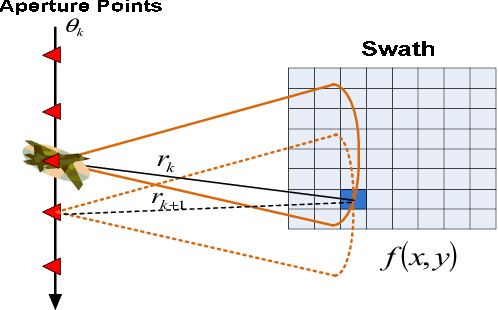
\includegraphics[width=0.5\linewidth]{src/rapport_complet/img/recouvrement_BP.png}
    \caption{Représentation du recouvrement en RSO}
    \label{fig:recouvrement_BP}
\end{figure}

Sur la Figure \ref{fig:recouvrement_BP}, on observe que, en raison du déplacement du drone et de l'ouverture de son antenne, certaines cellules au sol sont éclairées à plusieurs reprises le long de la trajectoire. 

Techniquement, l'algorithme standard de Backprojection, pour chaque pixel, corrige uniquement la phase selon l'expression (\ref{eq:correction_bp})

\begin{equation}
    \label{eq:correction_bp}
    I(\Vec{p})=\sum_m s_{RC}(r_{\Vec{p}, m})e^{-j\varphi_{e}(r_{\Vec{p}, m})}
\end{equation}
Avec: 
\begin{description}
    \item{$s_{RC}(u_{m})$: Le signal reçu à une distance $u_{r}$ [m]}
    \item{$\varphi(u_{m})$: La phase attendue pour un signal à la distance $u_m$ [rad]}
\end{description}
\vspace{1em}
Le terme $\varphi_e$ représente la correction de phase. 
La distance $r_{\Vec{p}, m}$ est une distance euclidienne. Par conséquent, cet algorithme ne réalise pas d'hypothèses sur la trajectoire du porteur. Dans le cadre de notre application, considérer une trajectoire quelconque est un grand avantage. 

Bien que cet algorithme soit conceptuellement simple, il est computativement exigeant, car il nécessite de parcourir chaque pixel de la scène et chaque position du radar. Cet algorithme a une complexité en $O(N^3)$. \\
Cependant, sa robustesse et sa capacité à produire des images précises en font une référence pour les applications SAR, notamment lorsque la trajectoire du radar est irrégulière. Cette robustesse vient du fait que les erreurs de phase locales sont « réintégrées » dans la somme temporelle, de sorte que leur impact reste spatialement localisé plutôt que global.
